\begin{mybilan}

	
	

	\begin{itemize}
		\item Dans une \kw{centrale thermique}, les combustibles fournissent une \kw{énergie thermique} qui produit la vaporisation de l'eau. La \kw{vapeur d'eau} en mouvement fournit de l'\kw{énergie mécanique} à la turbine et l'alternateur la transforme en \kw{énergie électrique}.
		%\item Une partie de l'énergie mécanique est <<perdue>>; elle n'est pas convertie en énergie électrique.
		\item Les centrales thermiques sont alimentées par des \kw{sources d'énergie fossiles}, non renouvelables. 
	\end{itemize}

	\begin{center}
		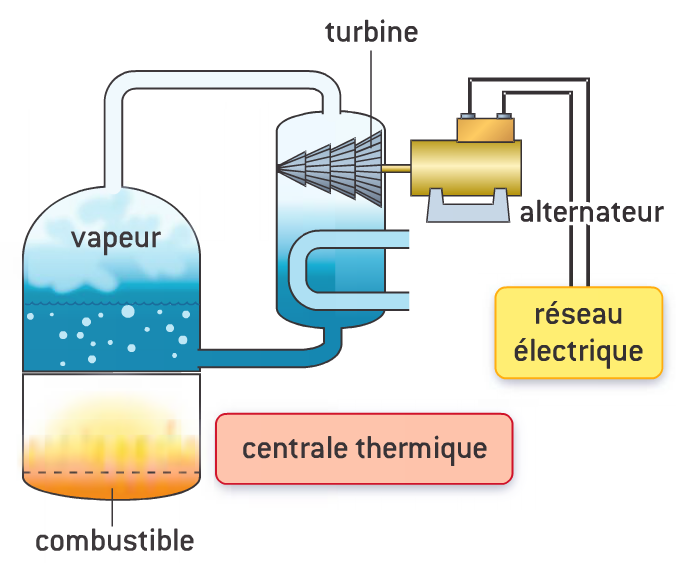
\includegraphics[scale=0.4]{centrale_thermique}
	\end{center}
\end{mybilan}